\documentclass{article}
\usepackage{122}

\usepackage{pgfplots}

\title{Теория вероятности \\ Домашнее задание №3}
\author{\AA{AAAAA AAAAAAA}{4} \\ \AA{AAAAAA}{11} \\ Вариант 3}

\begin{document}
  \maketitle

  \setcounter{section}{4}
  \section{Случайная величина $(\xi,\, \eta)$ распределена по нормальному закону с математическим ожиданием $(-0.15,\, 0)$ и ковариационной матрицей \\ $\Sigma = \begin{pmatrix}2 & 1\\1 & 1\end{pmatrix} $. Найти $P(\xi-\eta > 0)$}
  $$ \xi-\eta = \mathcal{N}\l(E\l(\xi-\eta\r),\, \mathcal{D}\l(\xi-\eta\r)\r) $$
  $\ds E\l(\xi-\eta\r) = E(\xi) - E(\eta) = -0.15$ \\
  $\ds \mathcal{D}\l(\xi-\eta\r) = \mathcal{D}(\xi) + \mathcal{D}(\eta) - 2 \operatorname{cov}\l(\xi,\, \eta\r) = 2 + 1 - 2 = 1$ \\
  $\ds \xi-\eta = \mathcal{N}\l(-0.15,\, 1\r)$ \\
  $\ds P(\xi-\eta > 0) = P(\mathcal{N}\l(0,\, 1\r) > 0.15) = 0.5 - \text{Ф}_0(0.15) = 0.5 - 0.0596 = \fbox{0.4404}$

  \section{Для заданной выборки}
  % [20.5, 15.0, 21.5, 20.0, 19.0, 21.5, 19.0, 19.0, 24.0, 28.0, 24.0, 28.0, 24.0, 25.0, 29.0, 25.0, 28.0, 37.5, 26.0, 29.0, 23.4, 12.6, 20.6, 27.0, 23.2, 22.6, 28.5, 23.0, 27.2, 25.2, 21.0, 24.2, 24.2, 24.2, 25.2, 21.6, 21.0, 21.6, 20.8, 22.2, 30.2, 25.0, 28.0, 25.0, 27.0, 17.4, 25.8, 24.2, 23.2, 21.2, 26.6, 27.0, 31.0, 33.4, 26.0, 27.0, 21.6, 30.2, 22.8, 26.4, 25.8, 25.2, 29.0, 25.0, 25.2, 25.2, 25.0, 27.3, 20.4, 22.7, 21.0, 26.0, 20.0, 21.6, 24.0, 22.0, 27.0, 24.2, 25.8, 26.2, 30.0, 31.0, 25.0, 26.2, 20.6, 25.2, 23.0, 25.0, 27.0, 25.1, 22.0, 29.2, 24.0, 30.0, 24.5, 21.5, 29.0, 23.4, 23.5, 25.9, 22.6, 25.0, 30.0, 30.2, 32.6, 23.8, 39.2, 25.0, 27.2, 25.6, 23.4, 26.2, 21.9, 26.9, 23.6, 26.9, 23.1, 19.9, 23.4, 19.2, 14.4, 20.7, 29.2, 21.9, 21.0, 21.9, 30.0, 22.6, 24.6, 24.1, 20.6, 27.8, 22.7, 23.4, 21.6, 24.6, 21.9, 23.8, 27.2, 34.0, 25.4, 23.2, 27.7, 23.0, 30.0, 25.1, 22.7, 27.8, 27.0, 22.6, 20.7, 19.4, 21.4, 23.0, 21.0, 24.3, 23.0, 23.2, 29.2, 24.4, 24.4, 21.8, 29.4, 30.0, 29.7, 29.2, 23.0, 23.4, 23.0, 25.9, 24.6, 22.6, 29.2, 23.4, 28.8, 25.4, 23.8, 30.0, 27.8, 21.0, 28.6, 27.2, 23.1, 26.9, 25.9, 24.2, 31.2, 25.9, 23.1, 27.6, 26.2, 22.2, 25.9, 27.6, 20.0, 27.0]
  $$ N = 196 $$

  \subsection{построите вариационный ряд выборки}
  $$
    \begin{array}{|c|c||c|c||c|c||c|c||c|c|}
      \hline
      12.6 & 1 & 21.2 & 1 & 23.5 & 1 & 25.8 & 3 & 28.6 & 1 \\
      14.4 & 1 & 21.4 & 1 & 23.6 & 1 & 25.9 & 5 & 28.8 & 1 \\
      15.0 & 1 & 21.5 & 3 & 23.8 & 3 & 26.0 & 3 & 29.0 & 4 \\
      17.4 & 1 & 21.6 & 5 & 24.0 & 5 & 26.2 & 4 & 29.2 & 5 \\
      19.0 & 3 & 21.8 & 1 & 24.1 & 1 & 26.4 & 1 & 29.4 & 1 \\
      19.2 & 1 & 21.9 & 4 & 24.2 & 6 & 26.6 & 1 & 29.7 & 1 \\
      19.4 & 1 & 22.0 & 2 & 24.3 & 1 & 26.9 & 3 & 30.0 & 7 \\
      19.9 & 1 & 22.2 & 2 & 24.4 & 2 & 27.0 & 8 & 30.2 & 3 \\
      20.0 & 3 & 22.6 & 5 & 24.5 & 1 & 27.2 & 4 & 31.0 & 2 \\
      20.4 & 1 & 22.7 & 3 & 24.6 & 3 & 27.3 & 1 & 31.2 & 1 \\
      20.5 & 1 & 22.8 & 1 & 25.0 & 10 & 27.6 & 2 & 32.6 & 1 \\
      20.6 & 3 & 23.0 & 7 & 25.1 & 2 & 27.7 & 1 & 33.4 & 1 \\
      20.7 & 2 & 23.1 & 3 & 25.2 & 6 & 27.8 & 3 & 34.0 & 1 \\
      20.8 & 1 & 23.2 & 4 & 25.4 & 2 & 28.0 & 4 & 37.5 & 1 \\
      21.0 & 6 & 23.4 & 7 & 25.6 & 1 & 28.5 & 1 & 39.2 & 1 \\
      \hline
    \end{array}
  $$

  \subsection{пользуясь формулой Стерджесса, определите количество интервалов разбиения выборки}
  $$ n = 1+\lfloor \log_2 N \rfloor $$
  почему-то все записывают это через десятичный логарифм,
  который, во-первых, брать сложнее чем двоичный (он есть в меньшем количестве языков/калькуляторов),
  и, во-вторых, там появляется mysterious число $3.322$, которое на самом деле $\ds \f{1}{\log_{10}(2)}$,
  но это некому непонятно. \\
  но ладно $\ds n = 1+ \lfloor 7.614 \rfloor = 8 $

  \subsection{постройте таблицу статистического ряда, в первой строке которой указаны интервалы разбиения, а во второй-частоты попадания элементов выборки в соответствующие интервалы}
  $$ \min = 12.6 $$
  $$ \max = 39.2 $$
  $$ d = \f{max-min}{N} = \f{39.2-12.6}{8} = 3.325 $$
  $$
    \begin{array}{|c|c|c|c|c|c|c|c|}
      \hline
      % [12.6,\, 15.925) & [15.925,\, 19.25) & [19.25,\, 22.575) & [22.575,\, 25.9) & [25.9,\, 29.225) & [29.225,\, 32.55) & [32.55,\, 35.875) & [35.875,\, 39.2] \\ \hline
      12.6 \text{-} 15.925 & 15.925 \text{-} 19.25 & 19.25 \text{-} 22.575 & 22.575 \text{-} 25.9 & 25.9 \text{-} 29.225 & 29.225 \text{-} 32.55 & 32.55 \text{-} 35.875 & 35.875 \text{-} 39.2 \\ \hline
      % \f{3}{196} & \f{5}{196} & \f{38}{196} & \f{78}{196} & \f{52}{196} & \f{15}{196} & \f{3}{196} & \f{2}{196} \\
      0.01531 & 0.02551 & 0.19388 & 0.39796 & 0.26531 & 0.07653 & 0.01531 & 0.01020 \\
      \hline
    \end{array}
  $$

  \subsection{постройте гистограмму}
  \begin{center}
    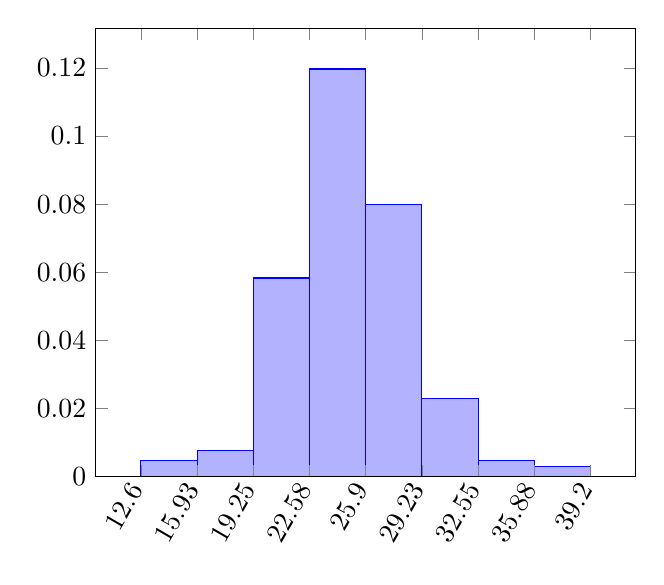
\begin{tikzpicture}
      \begin{axis}[ymin=0, area style,
        xtick={12.6, 15.925, 19.25, 22.575, 25.9, 29.225, 32.55, 35.875, 39.2},
        x tick label style={anchor=east,rotate=60,},
        yticklabel style={/pgf/number format/fixed},
      ]
        \addplot+[ybar interval,mark=no] plot coordinates{
          (12.6, 0.01531/3.325) (15.925, 0.02551/3.325) (19.25, 0.19388/3.325) (22.575, 0.39796/3.325) (25.9, 0.26531/3.325) (29.225, 0.07653/3.325) (32.55, 0.01531/3.325) (35.875, 0.01020/3.325) (39.2, 0.01020/3.325)
        };
      \end{axis}
    \end{tikzpicture}
  \end{center}

  \subsection{найдите реализации точечных оценок математического ожидания и дисперсии}
  $$ E = \sum \text{середина отрезка} \cdot \text{частота} $$
  $$ \mathcal{D} = E\l(\xi^2\r) - E\l(\xi\r)^2 $$
  $\ds E = \text{сложно я считал на питоне} = 26.6125 $ \\
  $\ds \mathcal{D} = 722.1575 - 26.6125^2 = 13.9323 $

  \subsection{на основе анализа результатов наблюдений выдвинете гипотезу о виде закона распределения наблюдаемой случайной величины}
  это похоже на фишера, потомучто выглядит как заострённый гаусс

\end{document}
